\documentclass{article}

\usepackage{graphicx}
\usepackage{amsfonts}

% Memory address
\newcommand\code[1]{{\tt #1}}
\newcommand\boldcode[1]{\code{#1}}
\newcommand\hex[1]{{\tt 0x#1}}
\newcommand\hexrange[2]{\hex{#1}{\tt -}\hex{#2}}

% Document
\begin{document}

\title{Peer-to-Peer 6502 Cellular Automata}
\author{Ian Holmes \\ Berkeley, California, USA}

\maketitle


\begin{abstract}
  As a toy example of incentivized, distributed spatial computation,
  this paper develops a blockchain for cellular automata
  comprising a 3D array of virtual 6502 processors, each with access to one page (256 bytes) of persistent storage,
  as well as the pages of its neighbors (and a read-only operating system).
  Simulation of this machine is incentivized via mining,
  writes are limited by transaction fee,
  and communications between adjacent nodes on the 3D grid are modeled as blockchain mergers.
\end{abstract}

\section{Introduction}

Cellular Automata (CA) are a common model for universal computation.
The idea that every pixel (or voxel) of the world computes and talks to its neighbors
is an appealing synthesis of concepts from natural science such as time- and space-invariance, and wave propagation.
Cellular automata, along with agent models, lattice gases, and other discretized frameworks, have been useful models in physics and biology,
and have also been used in computer games and artificial life experiments (A-Life).

Although straightforward to implement, cellular automata experiments are limited by the resources available to an individual;
furthermore, there are no well-established ways to bridge different experiments, for example to make a link between separate CA worlds.
Here, we describe a way to do this using the distributed timestamp service provided by a proof-of-work blockchain.

The cellular automata we develop as a motivating example are both universal and familiar, consisting of a three-dimensional grid of 6502 microprocessors broken into blocks.
The blockchain framework incentivizes simulation of individual chunks of cells, as well as traffic between chunks.

\subsection{Why 6502s?}

I chose the 6502 processor as the virtual machine for several reasons.
First, I like it, and so do many others, which is probably why it still gets attention 40 years after it appeared \cite{JonasKording2017}.
Second, it's simple, and compact (a slim memory footprint per cell is important for a CA; for example, 32 bits per instruction is too much).
Why not use RedCode, the programming language of Core War \cite{Dewdney1984}?
Core War is well-established among afficionados, and is studied by A-Life researchers \cite{VowkWaitSchmidt2004},
but it's poorly suited to spatially mapped simulations, since Core War programs run in a linear memory space.
Other prior A-Life frameworks have used virtual machines derived from 80x86 processors, as in Avida \cite{AdamiBrown1994}.

To define a new virtual machine with sufficient precision, it's helpful to stay close to a machine that physically exists.
We use 6502s with a very small set of machine extensions that are all memory-mapped, rather like hardware might be on a real 6502 system.

\subsection{Why blockchains?}

The blockchain was introduced as a distributed ledger for cryptocurrencies \cite{Nakamoto2008}.
More generally it can be used to drive computation on a distributed virtual machine.
In the Ethereum network, the virtual machine is used to implement smart contracts.
The use here is much simpler: the simulation of a virtual world of generic cellular automata.

It's certainly possible to run these automata on a centralized service, without using a blockchain.
The main role that the blockchain plays is to establish a consensus for distributed simulation.

The framework developed here is intended for recreational purposes: the coins mined by the system
have no ostensible purpose other than regulating the rate at which participants can write to the simulated world.
They might play the role of a score in a game world, measuring the contribution of the owner to keeping the world running.
However, alternate scores and success metrics are possible in the world we describe, such as the fitness of a user's programs.

\section{Methods}

\subsection{Chunks of cells}

Every cell of the cellular automata has a unique integer 3-space co-ordinate $(x,y,z) \in \mathbb{Z}^3$.

A single {\bf chunk} of the cellular automata is a $L \times L \times L$ cubic array of cells,
located at a base offset $L\alpha$,
where $\alpha = (\alpha_x,\alpha_y,\alpha_z)$ is an integer 3-vector called the {\bf chunk location}.

Cells in the chunk are indexed $(x,y,z$) where
$L\alpha_x \leq x < (L+1)\alpha_x$,
$L\alpha_y \leq y < (L+1)\alpha_y$,
$L\alpha_z \leq z < (L+1)\alpha_z$.

\subsection{Read-only and random-access storage}
\label{sec:Storage}

In designing general cellular automata running virtual machines,
it is useful to distinguish between a cell's read-only memory (ROM)
and its random-access memory (RAM).
The former is useful for storing the cell's operating program (or immutable parts of it); the latter, for tracking its internal state.

We allow cells to have both types of memory, RAM (for mutable state) and ROM (for immutable behavior).
It is perfectly possible to write cells with only one type of memory.
As an analogy, automata without ROM are like programs that run in user space without calling the operating system; they are by necessity small and simple.
Automata without RAM are like stateless protocols: they scale well, but they may be inflexible for some purposes.

Each cell has 256 bytes (one page) of updatable state (RAM).
All cells' bytes are initially zero
(including, implicitly, cells whose coordinates are outside the chunk; see also Section~\ref{sec:NeighborChunks}).
These bytes are the storage of the virtual machine.

Each cell also has a 32-kilobyte read-only operating system (ROM).
Most cells share the same operating system, and operating system changes should be rare,
so the O/S for a cell can be represented using a compact hash key such as SHA-256.

\subsection{Updating the chunk}
\label{sec:UpdatingChunk}

An {\bf update} of the chunk consists of updating $L^3$ uniformly-random selected cells in a well-defined pseudorandom order.
A Mersenne Twister (MT19937),
seeded on the tuple $(\alpha,L,U)$ where $U$ is the number of updates,
is a suitable random number generator (RNG) for this
and for generating the random cycle limit \code{STOPTIME} (Section~\ref{sec:Timeouts}),
which also must be generated for every updated cell.

Section~\ref{sec:NeighborChunks} describes a variant of this procedure whereby we construct a larger,
virtual chunk (including neighboring chunks) in order to perform predictive simulation of the neighborhood.

\subsection{Virtual machine}

A cell $(x,y,z)$ is updated by emulating a virtual machine.
In designing this virtual machine we want to use a well-known, simple architecture with small programs,
that is transparently universal.
The interface between the virtual machine and the chunk storage
needs to be such that the cell's ROM and the RAM, as well as the RAM of its neighbors,
are accessible to the code running in the virtual machine.

After some experiments with 32-bit ARM RISC architectures,
I settled on the 8-bit MOS Technology 6502 processor for a CPU.
The corresponding 16-bit memory map is shown in Table~\ref{tab:MemoryMap}.

In this memory map, the 27 pages of storage
for the cell and its 26 neighbors
in the $3 \times 3 \times 3$ unit cube centered on $(x,y,z)$
(in cellular automata terminology, the {\em three-dimensional Moore neighborhood}, shown in Figure~\ref{fig:UnitCube})
are mapped directly to bytes in the address range \hexrange{4000}{7FFF} of the virtual machine.
The detailed description of this part of the memory map
is given in Table~\ref{tab:MooreNeighborhood}.

The Moore neighborhood memory map can be understood as the cell $(x+i-1,y+j-1,z+k-1)$
mapping to page number (64+i*16+j*4+k) with $i,j,k \in \{0,1,2\}$.
Thus, in a memory-mapped 16-bit address, the bits have the interpretation shown in Table~\ref{tab:AddressBits}.
Note the exception: cell $(x,y,z)$ is not mapped to page 85 (\hexrange{5500}{55FF})
because it is mapped to zero page (\hexrange{0000}{00FF}) instead.

\subsection{Timeline of a cell update}
\label{sec:Timeline}

At the beginning of an update,
the registers \code{A,X,Y} are initialized to zero,
all status flags (register \code{P}) are set to zero,
the stack pointer (register \code{SP}) is set to \hex{FF},
the program counter \code{PC} is set to \hex{0000},
the cellular automata states are copied into memory (to zero page and other pages shown in Table~\ref{tab:MooreNeighborhood}),
and execution begins at the first byte of zero page.

Execution is terminated
when a software interrupt or undefined instruction is encountered,
or by non-maskable interrupt after completion of the first instruction that takes the cycle count past \code{STOPTIME} cycles,
where \code{STOPTIME} is a 16-bit integer.
For notes on how \code{STOPTIME} is chosen, see Section~\ref{sec:Timeouts}.

On termination, the transient address ranges in the memory map
(including the stack) are discarded.
If execution was terminated by timeout, then the rest of memory is also discarded,
and the state of the CA is restored.
Otherwise, if the program exited (by software interrupt or undefined opcode) before timing out,
the neighborhood memory-mapped pages (zero page and other pages in the range \hexrange{4000}{7FFF}, see Table~\ref{tab:MooreNeighborhood})
are copied back to the cellular automata storage.

\subsection{Timeouts}
\label{sec:Timeouts}

We need to set a limit on how many cycles a program is allowed to run for (i.e. \code{STOPTIME}).
The problem is that, if we set a hard limit, randomly emergent programs will tend to hit that limit
(e.g. by entering infinite loops)
and human programmers will be tempted to surf close to it.

To encourage quicker programs,
we make \code{STOPTIME} a random variable, instead of a fixed limit.
We also require that programs exit gracefully (returning control to the emulator via a software interrupt)
if their changes are to be committed to storage.
As well as discouraging crashes and other CPU hogs, this makes it easier to write programs that are atomic (all-or-nothing) in their effects.
Programs can check the \code{TIME} timer at \hexrange{FFF6}{FFF7} to see how many cycles are available.

The random variable \code{STOPTIME} is generated using the chunk RNG (Section~\ref{sec:UpdatingChunk})
and the following algorithm:
\begin{itemize}
\item Let $r$ and $s$ denote random 16-bit integers
\item Let $z$ be the number of leading zero bits of $s$, so $0 \leq z \leq 16$
\item Let $m = \mbox{min}(z,13) + 2$. The distribution of $m$ is now given by
  \[
  P(m=k) = \left\{ \begin{array}{ll} 2^{1-k} & \mbox{if $2 \leq k < 15$} \\ 2^{-13} & \mbox{if $k = 15$} \end{array} \right.
  \]
\item Set \code{STOPTIME} to $(2^m \vee (r \wedge (2^m - 1))$
\end{itemize}

% This Perl one-liner calculates the mean value of STOPTIME and some related probabilities
% perl -e '$e=0;for($m=2;$m<=15;++$m){$p=($m<15?(2**(1-$m)):(2**(-13)));$b=2**$m;$s=($b+($b-1)/2);print"$p $t $s\n";$e+=$p*$s;$t+=$p}print"$t $e\n"'

The mean value of \code{STOPTIME} is 44.5 cycles,
but there is a small ($\sim$0.5\%) chance that it's over 1,000 cycles,
and an even smaller ($\sim$0.05\%) chance that it's over 10,000 cycles.

\subsection{Special addresses}

There are several emulator-mapped memory addresses that perform special functions:
the read-only \code{TIME} (\hexrange{FFF6}{FFF7}), which is the number of cycles until forced termination;
the write-only \code{SWAP} (\hex{FFF8}), which facilitates diffusion models;
and the read-only \code{RAND} (\hex{FFF9}), which provides a random number generator.

These are described in the sections below.

\subsection{Operating system updates}

The machine architecture described so far is adequate if the operating system ROM is shared by every cell in the chunk.
To allow O/S updates to be propagated across the chunk, we introduce two specific mechanisms.
Guiding the design of this mechanism are the following two principles:
\begin{itemize}
\item If a cell writes another cell's RAM, then it should expect that cell's ROM to be the same as its own.
\item Cells should, nevertheless, be allowed to diffuse past each other without necessarily overwriting each others' ROM.
\end{itemize}

The first mechanism for O/S propagation is the write-only \code{SWAP} address, \hex{FFF8}.
Any value written to \code{SWAP} is interpreted as the index of a neighboring cell.
Only the lower 6 bits of the written byte are relevant, and specify a cell in the $3 \times 3 \times 3$ Moore neighborhood
in the same way as bits 8-13 of a memory-mapped storage address (c.f. Table~\ref{tab:AddressBits}).

Writing a byte to \code{SWAP} has the effect of swapping the storage and operating system pages associated with the current cell and the specified neighboring cell,
and then triggering a software interrupt, terminating execution.
If the neighboring cell is outside the chunk,
this updates the current cell (and its operating system) but has no effect on the neighboring cell
(although see Section~\ref{sec:NeighborChunks}).
If the written byte is not a valid index byte, then there is no effect.
A software interrupt is triggered, and program execution terminated, regardless of whether the written byte is a valid index pointing to a cell within the chunk.

Reading a byte from address \code{SWAP} always yields zero, and has no other effect.

As mentioned above, the \code{SWAP} interface is one of two mechanisms by which operating system code is propagated across the chunk.
The second mechanism is built into the memory-mapped storage interface itself.
During an update, writing any byte to any neighboring cell, i.e. any cell in the memory-mapped storage (\hexrange{4000}{7FFF}),
has the implicit effect of copying the operating system pages from the current cell to the neighbor.
This is handled transparently by the emulator without consuming any additional cycles.

\subsection{Random numbers}

The read-only \code{RAND} address, \hex{FFF9}, is a random number generator.
Reading a byte from \code{RAND} yields 8 random bits, newly sampled with each read (i.e. multiple reads yield different results).

The random numbers are provided by an RNG seeded on the cell and chunk co-ordinates and the chunk update count
(NB this is a per-cell RNG, distinct from the per-chunk RNG of Section~\ref{sec:UpdatingChunk} that selects cells and sets \code{STOPTIME}).

\subsection{Timer}

The read-only 16-bit \code{TIME} address, \hexrange{FFF6}{FFF7}, gives the number of cycles before the program is terminated.
(More precisely, this address is initialized to \code{STOPTIME} before the first instruction is executed,
and decremented after completion of each instruction.)

\subsection{Neighboring chunks}
\label{sec:NeighborChunks}

Two $L$-sized chunks are neighbors if their chunk locations are neighbors;
that is, they have base offsets $L\alpha_1$ and $L\alpha_2$,
and $\alpha_1$ is in the Moore neighborhood of $\alpha_2$.
This is equivalent to the statement that (at least) one cell in the first chunk has (at least) one cell in the second chunk in its Moore neighborhood, and vice versa.

When running several updates of the central chunk,
given some knowledge (e.g. a recent snapshot) for the state of neighboring chunks,
and assuming that communication with those neighboring chunks is imperfect (so that our snapshot may be out of date),
we perform {\bf predictive simulation} of neighboring chunks.

Specifically, when updating the central chunk, we also update our estimates of the neighboring chunks.
To do this we construct a $(3L) \times (3L) \times (3L)$ virtual {\bf super-chunk},
into which is mapped the current state of our chunk, as well as our current best estimates of the 26 neighboring chunks.

We then update all 27 sub-chunks of the $3 \times 3 \times 3$ unit cube in the usual order ($z$-fastest, like the MSB in Table~\ref{tab:AddressBits}).
Each sub-chunk's update is handled as though it were a single chunk,
using the algorithm of Section~\ref{sec:UpdatingChunk},
i.e. updating $L^3$ cells selected using a random number generator seeded with the tuple $(\alpha',L,U')$
where $\alpha'$ is the neighboring chunk location and $U'$ is our estimate of the neighboring chunk update count
(which is updated along with our estimate of the neighboring chunk states).

Writes between neighboring chunks are not discarded, as they were previously
(though writes outside of the $(3L) \times (3L) \times (3L)$ chunk will still be discarded).
However, the central block's estimates of the state of its neighboring chunks
may be overwritten in the future by news from those neighboring chunks,
arriving in the blockchain in the form of neighboring segments (Section~\ref{sec:NeighboringSegments}).

Predictive simulation facilitates traffic between chunks
by allowing migration to be an active process, instead of a passive diffusion at the border.

\subsection{Blockchain}
\label{sec:Blockchain}

The chunk has an associated blockchain, defined as in \cite{Nakamoto2008}.
Updates are incentivized by mining,
and the reward for mining is adjusted to include redemption of coins mined by neighboring cell-chunk blockchains
(this also updates the boundaries with those chunks).

\subsection{Driving updates with the blockchain}
\label{sec:ProofOfWork}

A valid block must include a full description of the state of the $L^3$ cells in the central chunk,
and the new best estimates for the $26L^3$ cells in neighboring chunks,
following $C$ updates of the super-chunk described in Section~\ref{sec:NeighborChunks}.
$C$ is the number of cycles per cell expected in the blockchain update time
(which for bitcoin is 10 minutes).

Let the definition of a block include the coordinates $(\alpha_x,\alpha_y,\alpha_z,L,U)$
used to seed the chunk's random number generator and identify the chunk in space and time,
as well as the estimated update counts for neighboring chunks.

\subsection{Write operations}

Any transaction in the blockchain may include, as additional data,
a {\bf write operation} which modifies the state of one or more cells of the chunk.
This modification is considered to take place after the emulation of $C$ update cycles
which is part of the proof-of-work protocol (Section~\ref{sec:ProofOfWork}).

The order in which such write operations are applied,
each potentially overwriting the state modifications of its predecessors,
is implied by the ordering of the transaction in the block.
As usual, the transaction may include network fees to incentivize inclusion of transactions
by the miner
(and prioritization later in the block).
The transaction fee is, as usual, the difference between the output and input values of the transaction,
minus a write operation tax of $W$ coins per cell written,
to discourage frivolous edits.
If (for example) $W=1$, then minting a coin lets you write a cell.

As well as writing the (volatile) state of the cell, a write operation can overwrite the cell's 32K operating system
(mapped to address range \hexrange{8000}{FFEF} in the virtual machine; the last 16 bytes, corresponding to \hexrange{FFF0}{FFFF}, are ignored).
After the first time an operating system is used in the blockchain, it can be referred to by SHA-256 hash, to save space.

\subsection{Neighboring segments}
\label{sec:NeighboringSegments}

The block may include sections of blockchain from neighboring chunks,
referred to as {\bf neighboring segments}.

Neighboring segments must be consistent continuations of any previously-observed neighboring segments
earlier on the central blockchain.
They may, themselves, recursively refer to parts of the current blockchain as their own neighboring segments,
summarized by their hashes for compactness.

When a block includes an neighboring segment, the chunk's estimate for that neighboring chunk's state is updated to match the information in the neighboring segment.
Regular mutual inclusion of neighboring segments from neighboring chunks' blockchains
corresponds to keeping a bidirectional read-only interface open between those chunks.

To incentivize this bidirectional traffic,
inclusion of an neighboring segment in a block for the first time
accrues an additional benefit of $C/R$ coins to the miner of the block,
where $C$ is the number of {\bf redeemable coins} mined or accrued (via transitive neighbor relationships)
by cells in the neighboring chunk,
and $R$ is the {\bf redemption rate}, the number of redeemable coins in neighboring chunks
required to accrue a coin in the current chunk.
It is of course necessary to have $R>2$ to prevent an explosion of redeemable value in 3D space;
a conservative value is $R=26$, which (in the densely-connected Moore neighborhood)
ensures that the number of coins redeemed is less than the number of coins mined locally
(the corresponding value for the von Neumann neighborhood of Table~\ref{tab:VonNeumannNeighborhood}
is much lower, at $R=6$).

\subsection{Parameters}

Setting the parameters $L$ (chunk size) and $C$ (updates per block)
is a little arbitrary, but can be guided by target memory footprint and clock rate.
For memory, the chunk state requires $256 \times L^3$ bytes.
For clock rate, if we ran a 6502 CPU at 1Mhz for 10 minutes, with a mean of $44.5$ cycles per cellular update,
we would update the whole chunk $10^6 \times T / (44.5 \times L^3)$ times
where $T$ is the time in seconds between blocks ($T=36,000$ for bitcoin).
Faster clocks and protocols no doubt allow better numbers,
but considering these values and estimating conservatively,
we recommend $L=64$ and $C=4$ so that
each cell is updated every few minutes;
each block takes at most 64Mb to describe the chunk state;
and the computational burden is roughly comparable to a 6502 CPU.

% Tables, macros
% Macro to generate neighborhood memory map table
\newcommand\memtable[1]{
\begin{tabular}{rlll}
  \hline
  Label & From & To & Contents \\
  \hline
  #1
  \hline
\end{tabular}
}

\newcommand\memrow[5]{
    \boldcode{#5} & \hex{{#1}00} & \hex{{#1}FF} & State of cell $(x#2,y#3,z#4)$ \\
}

% The \memxyz macro gives a densely-connected (von Neumann) neighborhood
\newcommand\memz[6]{
  \memrow{#1}{#4}{#5}{-1}{D#6}
  \memrow{#2}{#4}{#5}{}{#6}
  \memrow{#3}{#4}{#5}{+1}{U#6}
}

\newcommand\memyz[3]{
  \memz{{#1}0}{{#1}1}{{#1}2}{#2}{-1}{S#3}
  \memz{{#1}4}{{#1}5}{{#1}6}{#2}{}{#3}
  \memz{{#1}8}{{#1}9}{{#1}A}{#2}{+1}{N#3}
}

\newcommand\memxyz{
  \memyz{4}{-1}{W}

  %  \memyz{5}{} includes zero page-mapped cell (x,y,z), which we want to skip, so spell it out without that
  \memz{50}{51}{52}{}{-1}{S}
  \memrow{54}{}{}{-1}{W}
  \memrow{56}{}{}{+1}{E}
  \memz{58}{59}{5A}{}{+1}{N}

  \memyz{6}{+1}{E}
}

% The following table is a sparse neighborhood (von Neumann, 6 neighbors/cell)
\newcommand\vonneumannmap{\memtable{
  \memrow{45}{-1}{}{}{W}
  \memrow{51}{}{-1}{}{S}
  \memrow{54}{}{}{-1}{D}
  \memrow{56}{}{}{+1}{U}
  \memrow{59}{}{+1}{}{N}
  \memrow{65}{+1}{}{}{E}
}}

% The following neighborhood is dense (Moore, 26 neighbors/cell)
\newcommand\mooremap{\memtable{\memxyz}}

% Captions
\newcommand\labeq[2]{\boldcode{#1}\code{=}\hex{#2}}
\newcommand\asslabels{
  The labels (\code{N}, \code{S}, \code{E}, \code{W}, \code{U}, \code{D} \ldots)
  are pre-defined in the assembler to the respective base addresses (\labeq{N}{5900}, \labeq{S}{5100}, and so on).
  The corresponding labels with \code{PAGE} appended
  are predefined to be the respective MSBs of those base addresses (\labeq{NPAGE}{59}, \labeq{SPAGE}{51}, and so on).
  The assembler also pre-defines the symbols
  \labeq{XDIR}{1000}, \labeq{YDIR}{0400}, \labeq{ZDIR}{0100};
  \labeq{XPAGE}{10}, \labeq{YPAGE}{04}, \labeq{ZPAGE}{01};
  \labeq{ORIG}{5500}, \labeq{ORIGPAGE}{55};
  \labeq{BASE}{4000}, \labeq{BASEPAGE}{40}.
}

% Tables
\begin{table}
\begin{tabular}{llll}
  \hline
  From & To & Type & Contents \\
  \hline
  \hex{0000} & \hex{00FF} & RAM (storage-mapped) & State of cell $(x,y,z)$ \\
  \hex{0100} & \hex{01FF} & RAM (transient) & Stack: initialized to zero \\
  \hex{0200} & \hex{03FF} & RAM (transient) & Scratch memory: initialized to zero \\
  \hex{0400} & \hex{3FFF} & ROM & Reserved: zero \\
  \hex{4000} & \hex{7FFF} & RAM (storage-mapped) & Memory-mapped neighborhood (Table~\ref{tab:MooreNeighborhood}) \\
  \hex{8000} & \hex{FFF0} & ROM & Operating system \\
  \hex{FFF0} & \hex{FFF5} & ROM & Reserved; zero \\
  \hex{FFF6} & \hex{FFF7} & Read-only & \code{TIME}: number of cycles left until termination \\
  \hex{FFF8} & \hex{FFF8} & Write-only & \code{SWAP}: write to swap cell with neighbor \\
  \hex{FFF9} & \hex{FFF9} & Read-only & \code{RAND}: random byte generator \\
  \hex{FFFA} & \hex{FFFF} & ROM & Reset and interrupt vectors: zero \\
  \hline
\end{tabular}
\caption{
  \label{tab:MemoryMap}
  Memory map for the 6502 virtual machine of cell $(x,y,z)$.
}
\end{table}

\begin{table}
\mooremap
\caption{
  \label{tab:MooreNeighborhood}
  Memory map for the 6502 virtual machine of cell $(x,y,z)$,
  using the 26-cell three-dimensional Moore neighborhood (Figure~\ref{fig:UnitCube}).
  All address ranges not defined in this table are read-only and zero;
  writing to these addresses has no effect.
  Pages mapping to cells outside the chunk (e.g. $x<L\alpha_x$ or $x \geq (L+1)\alpha_x$, or similarly for $y,z$)
  are read-only and zero (unless otherwise specified, as in Section~\ref{sec:NeighborChunks}).
  Writing to these addresses has no effect.
  \asslabels
}
\end{table}

\begin{table}
\vonneumannmap
\caption{
  \label{tab:VonNeumannNeighborhood}
  Memory map for the 6502 virtual machine of cell $(x,y,z)$,
  using the 6-cell three-dimensional von Neumann neighborhood.
  This memory map may be considered a subset of the memory map in Table~\ref{tab:MooreNeighborhood}.
  \asslabels
}
\end{table}

\begin{table}
\begin{tabular}{lll}
  \hline
  Byte & Bit(s) & Meaning \\
  \hline
  MSB & 4,5 & $i$ \\
  MSB & 2,3 & $j$ \\
  MSB & 0,1 & $k$ \\
  LSB & 0-7 & Address within page \\
  \hline
\end{tabular}
\caption{
  Interpretation of a 16-bit address in the memory-mapped range \hexrange{4000}{7FFF}
  as pointing to the cell $(x+i-1,y+j-1,z+k-1)$.
  See Table~\ref{tab:MooreNeighborhood} and Table~\ref{tab:VonNeumannNeighborhood}, and Figure~\ref{fig:UnitCube}.
  Note that $i,j,k, \in \{ 0,1,2 \}$.
  \label{tab:AddressBits}
}
\end{table}

\begin{figure}
  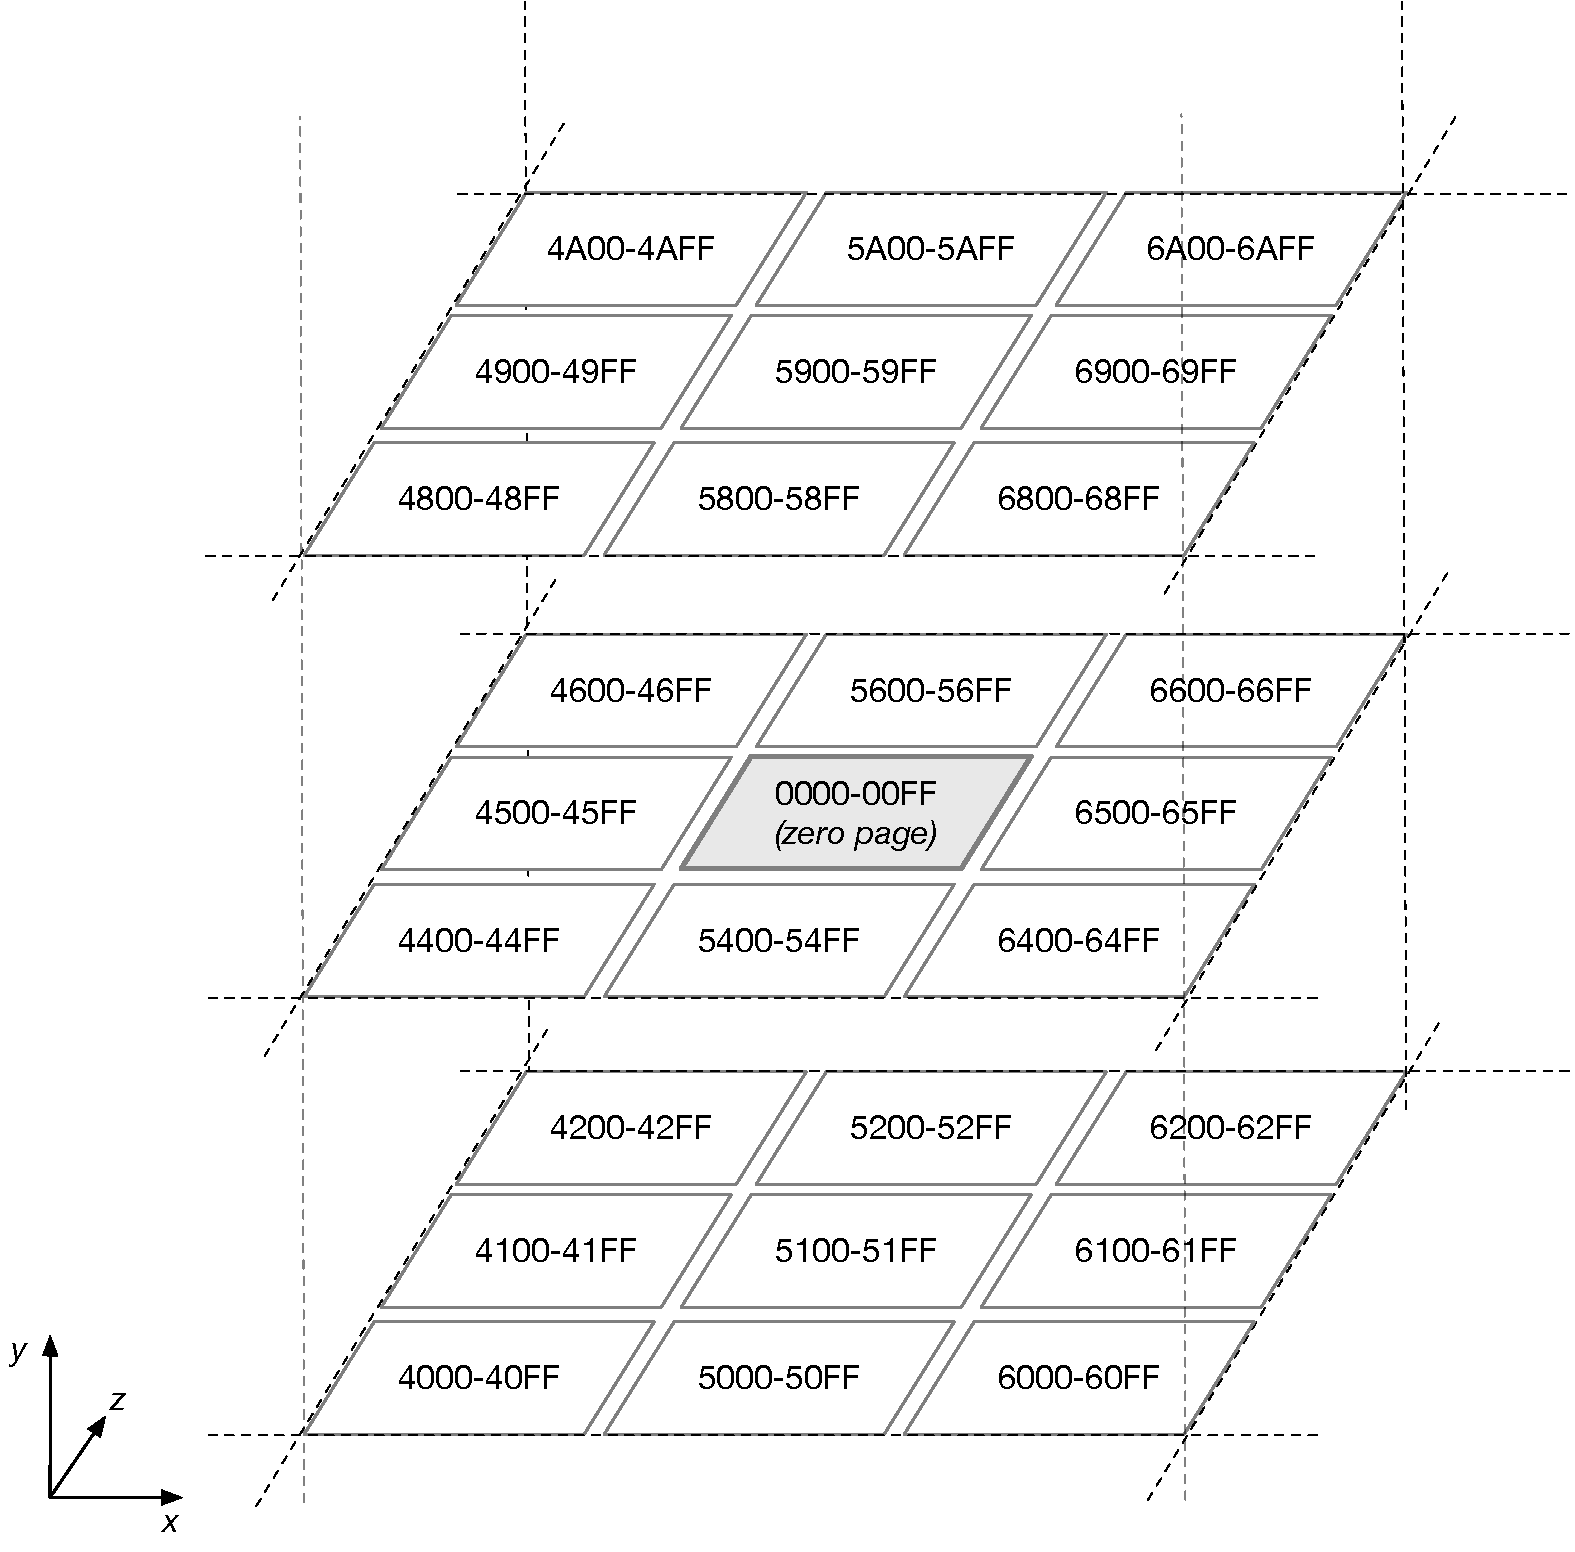
\includegraphics[width=\textwidth]{unitcube.pdf}
\caption{
  The memory-mapped neighborhood of a cell (see Table~\ref{tab:MemoryMap} and Table~\ref{tab:MooreNeighborhood}).
  The central cell is at $(1,1,1)$, and is mapped to zero page.
  All other cells are mapped to pages in the range \hexrange{4000}{7FFF},
  the first six bits of the address MSB corresponding to the $x$, $y$ and $z$ co-ordinates within this cell (see Table~\ref{tab:AddressBits}).
  \asslabels
  \label{fig:UnitCube}
}
\end{figure}

\section*{Acknowledgments}
Thanks to Peter Irvine, Chris Evans, Richard Evans, Michael Mateas.

\bibliographystyle{plain}
\bibliography{references}

\end{document}
